% !TeX spellcheck = en_EN-English
\documentclass[a4paper]{article}
\usepackage[slovak]{babel}
\usepackage[utf8]{inputenc}
\usepackage[T1]{fontenc}
\usepackage{a4wide}
\usepackage{amsmath}
\usepackage{amsfonts}
\usepackage{amssymb}
\usepackage{mathrsfs}
\usepackage[small,bf]{caption}
\usepackage{subcaption}
\usepackage{xcolor}
\usepackage{graphicx}
\usepackage{enumerate}
\usepackage{hyperref}



\pagestyle{empty}
\setlength{\parindent}{0pt}

\newenvironment{modenumerate}
{\enumerate\setupmodenumerate}
{\endenumerate}

\renewcommand{\thesubsection}{\thesection.\alph{subsection}}

\begin{document} 
	
	\pagenumbering{arabic}
	\pagestyle{plain}
	
	\begin{center}
		\sc\large
		PHYSICAL BASED ANIMATIONS AND MATHEMATICAL MODELING HW 1 
	\end{center}
	
	Autor: Marián Kravec
	\\
	\\
	This document contains only same information as comments in the code and pictures of final plot in case wolfram mathematica would behave strangely and will produce different plot during the marking.
	
	I was born September 18 so parameter $K_m$ is in my case $K_m=0.162$ ($18*9=0.162$)
	
	First let's do some things that will be useless, but I thought I would need them.
	\begin{align*}
		\text{We have 3 equations:}
		\\
		1. e(t)=s_p-\tau(t)
		\\
		2. V(t)=A_p*e(t)+A_d*e'(t)
		\\
		3. \tau'(t)=-K_p*\tau(t)-K_d*\tau'(t)+K_m*V(t)
		\\
		\text{First we compute derivative of 1. equation with respect to t and we get new equation:}
		\\
		4. e'(t)=\tau'(t)
		\\
		\text{Now we substitute $e'(t)$ and $e(t)$ in 3. equation using 1. and 4. equation}
		\\
		5. V(t)=A_p*(s_p-\tau(t))+A_d*\tau'(t)
		\\
		And finally we substitute V(t) in eqution 3. using equation 5.
		\\
		6. \tau'(t)=-K_p*\tau(t)-K_d*\tau'(t)+K_m*(A_p*(s_p-\tau(t))+A_d*\tau'(t))
	\end{align*}
	Now we have final version of our differential equation which we can input into NDSolve funtion provided in Wolfram to solve our equation with initial condition $\tau(0)=0$. Unfortunately when I tried to use just this final equation and initial condition it did not behaved as I expected (I was getting strange results compared to my classmate so in the end I input all three equation and initial condition into NDSlove function 
	\section{} 
	\subsection{}
	Our initial torque is given in assignment and it is $\tau(0)=0$
	Using this and 1. equation and setpoint $s_p=100$ we can compute initial error which is:
	$e(0)=s_p-\tau(0)=100-0=100$
	\\
	Next we compute value $V(0)$. Thankfully wolfram interpolated also this function so we just need to ask for it initial value (computing it by hand is not as straightforward as in case of initial error because in equation for voltage we have derivation of function) we get value $V(0)=9.98$.
	
	\subsection{}
	Plot of voltage:
	\\
	\centerline{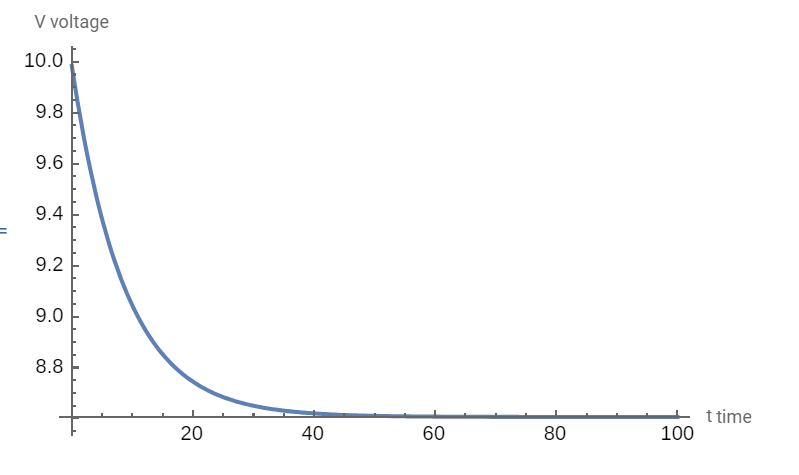
\includegraphics[width=0.8\textwidth]{1_b_v}}[h!]
	We can see that we start with input voltage around 10 which then slowly decline and after approximately 1 minute (60 seconds) it approach 8.6V
	
	\subsection{}
	Plot of torque:
	\\
	\centerline{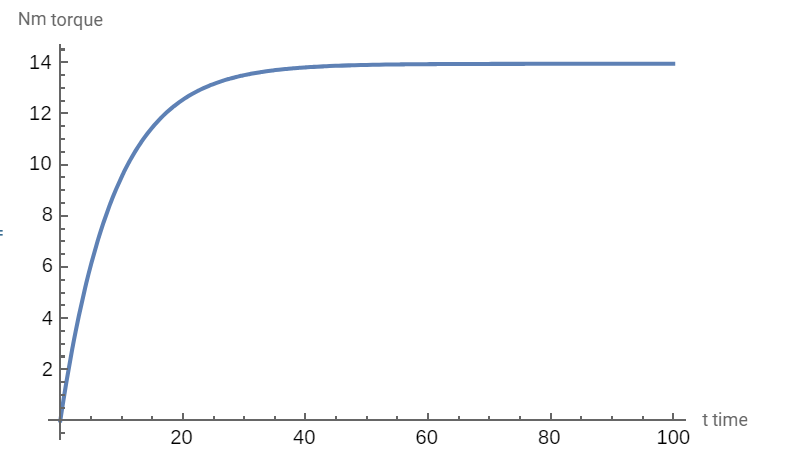
\includegraphics[width=0.8\textwidth]{1_c_t}}[h!]
	We can see that initial torque is 0 and it slowly increase. Around same time as voltage got to 0 (around 1 minute) we can see that torque seems to reach it maximum at around 14Nm.
	
	\section{}
	\subsection{}
	Value of voltage after 10 seconds (t=10s) we compute in a same way as we computed initial value, we get value $V(10)=9.04$.
	
	\subsection{}
	As we saw on plot in task 1 part (c) our motor seem to never reach the setpoing torque of 100Nm, it seems to reach at most 14Nm.
	
	\subsection{}
	On the same plot we can see that maximum torque is reaches after around 1 minute, however from theoretical perspective we can assume that it's approaching maximum so it will never reach it however after 1 minute it's already pretty close to it
	
	\subsection{}
	We compute votage and torque after one hour by evaluating them at t=3600. I decided to try two different approaches, one is to interpolate on interval $<0, 3600>$ (so value for $t=3600$ is interpolated) and other is to interpolate only on interval $<0, 100>$ (so value $t=3600$ is extrapolated) (In code first approach in place where it belong and second is at the of file).
	\\
	\\ 
	With first approach we can see that values stabilize after first minute.
	\\ 
	\centerline{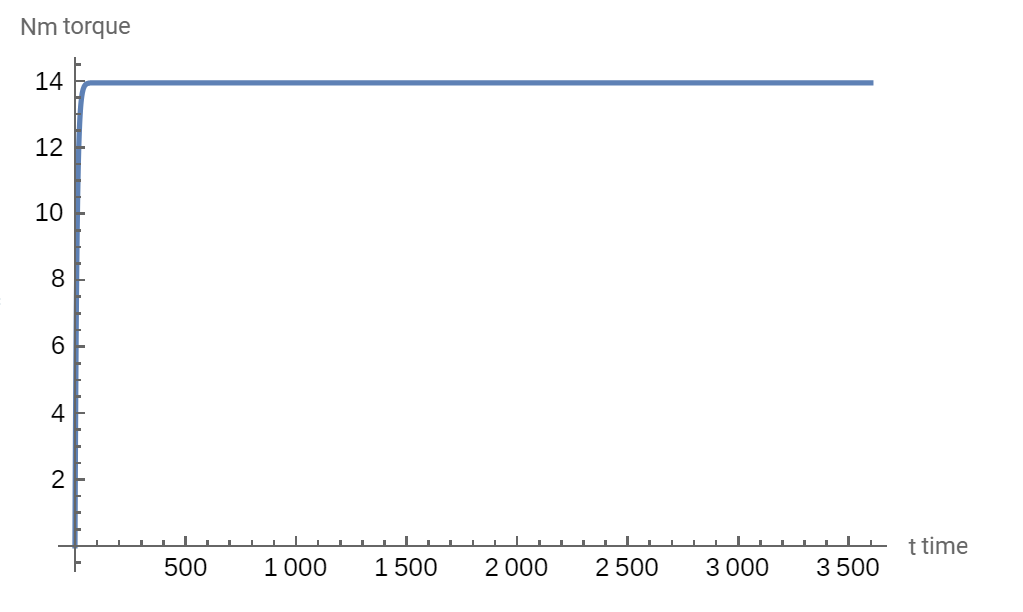
\includegraphics[width=0.8\textwidth]{2_d_t_1}}[h!]
	\centerline{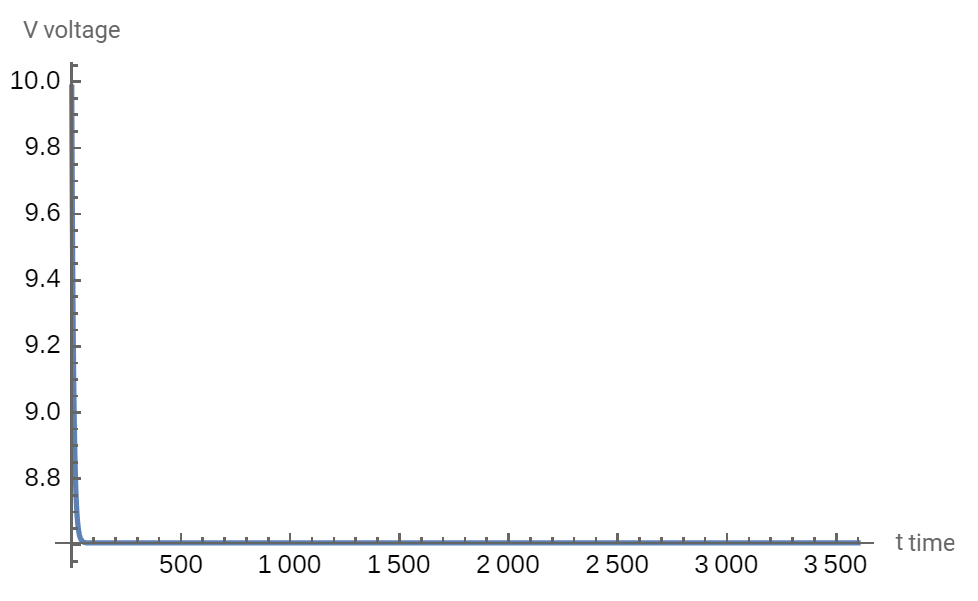
\includegraphics[width=0.8\textwidth]{2_d_v_1}}[h!]
	So after one hour torque is $\tau(3600)=13.94$ and voltage is $V(3600)=8.61$.
	\\
	With second approach we can see that values stops being stable after couple of minutes and starts to increase (torque) or decrease (voltage) significantly (seems like they will approach infinity) most likely caused by the fact that they are extrapolated.
	\\
	\centerline{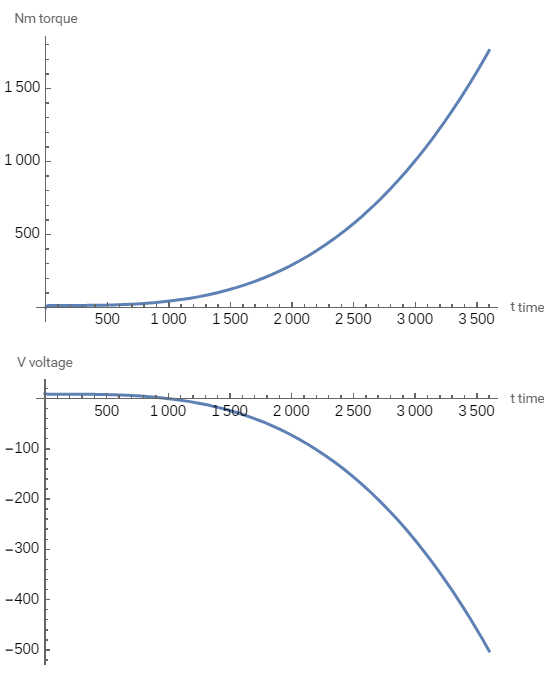
\includegraphics[width=0.8\textwidth]{2_d_vt_2}}[h!]
	So after one hour torque is $\tau(3600)=1760.42$ and voltage is $V(3600)=-502.09$.
	
	\section{}
	In my pursuit to find parameters such that torque would be described by periodic or chaotic function I tried multiple things such as trying to understand how this system works or trying to create for loop to go through multiple combinations at once (just by looking at final plot) (unfortunately I always got lot's of errors which I was not able to solve) or even rewriting it in python (which also did not help because I got different results in each language) so in the end I did it by trial and error.
	\subsection{}
	In the end I found combination of parameters that produced chaotic functions (described more in part (e)) and I was trying to fine tune it to find case when result looks periodic.
	
	In the end I got best results for these values: $K_p=0$, $K_d=-0.951621$, $\tau(0)=0$.
	\\
	\centerline{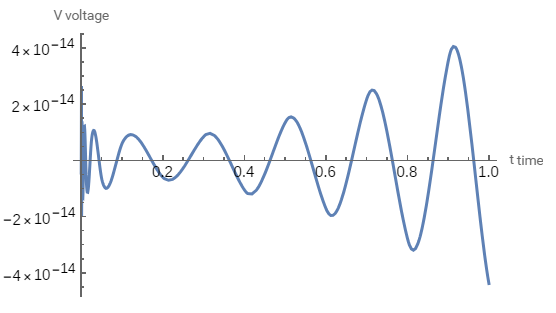
\includegraphics[width=0.8\textwidth]{3_a_v}}[h!]
	On plot of Voltage we can see that it for first 0.1 oscillate quickly and then oscillations slow down to period around 0.2 with increasing amplitude.
	
	\subsection{}
	Resulting plot of torque looks like this:
	\\
	\centerline{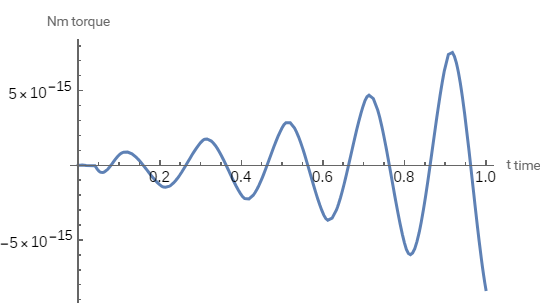
\includegraphics[width=0.8\textwidth]{3_b_t}}[h!]
	
	On torque plot we can see similar behavior to voltage however in this case we behavior during first 0.1 is similar to rest (it's not that visible on this plot but if zoom in we would see that it also periodic there with increasing amplitude) so it has period around 0.2 and increasing amplitude.
	
	\subsection{}
	Not in assignment.
	\subsection{}
	Not in assignment.
	
	\subsection{}
	After lot's of trial and error I found out that if we leave initial condition untouched and set proportional gain to $K_p=0$ we get quite chaotic behavior of our system for almost any value of derivative gain in interval $<-1,1>$ (except for 0)(it's chaotic also for bigger and smaller values of Kd but I am not sure up to which value or if for all values).
	Here is one example where behavior can be considered chaotic: $K_p=0$, $K_d=-0.375$, $\tau(0)=0$. 
	
	Resulting plot of voltage looks like this:
	\\
	\centerline{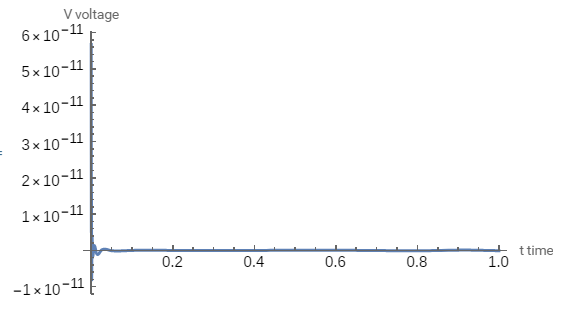
\includegraphics[width=0.8\textwidth]{3_e_v}}[h!]
	
	On plot of voltage we can see that it oscillate around zero, we can see that for first few milliseconds in acquires values up to $10^(-11)$ but then only up to $10^(-13)$. 
	\subsection{}
	
	Resulting plot of voltage looks like this:
	\\
	\centerline{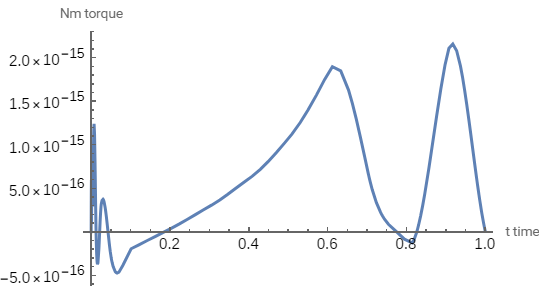
\includegraphics[width=0.8\textwidth]{3_f_t}}[h!]
	
	On plot of torque we can see that for first 0.1 second it oscillate around 0 then raise for next half of a second and then suddenly drops for next 0.2 seconds then raises and drop again, I think this can be considered chaotic behavior.
	
	\subsection{}
	Now we prepare two interpolations for our differential equation
	one with initial condition: 
	$\tau_1(0)=0.000000001$
	and second with initial condition:
	$\tau_2(0)=0.000000002$
	We interpolate both on interval $<0,10000>$ and then calculate $d_n=\tau_2(10000)-\tau_1(10000)$
	
	
	Now we want to compute $\lambda$ and we have equation:
	$dn=0.000000001*e^{10000*\lambda}$. Let's get value $\lambda$ from it:
	\begin{align*}
		d_n=0.000000001*e^{10000*\lambda} 
		\\
		ln(d_n)=ln(0.000000001*e^{10000*\lambda})
		\\
		ln(d_n)=ln(0.000000001)+ln(e^{10000*\lambda})
		\\
		ln(d_n)=ln(0.000000001)+ln(e^{10000*\lambda})
		\\
		ln(d_n)=ln(0.000000001)+10000*\lambda
		\\
		\lambda=(ln(d_n)-ln(0.000000001))/10000
	\end{align*}
	Now let's do two test first let's test whether system with original parameters is chaotic and then if system we cosidered chaotic in Task 3 part e) is really chaotic.
	
	When we do this computation for original system can see that even though we compute values with 40 decimal point precision we still get 0 difference, this would make however lambda undefined because there is no real exponent $x$ for which $e^x$ would be 0. However because we get same value for both initial conditions we can assume that our system is stable.
	
	Now let's try to do same computations for system that we considered chaotic in task 3 part e).
	In this case we get value $d_n\approx10^{-9}$, when we compute value $\lambda$ from this difference we get value $\lambda=-6.02*10^{-10}$. In this case we get small but negative Lyapunov exponent, which should mean that the distance between these two results should not increase indefinitely and the system should settle down just to see real behavior let's as a final thing plot these two $\tau$.
	\\
	\centerline{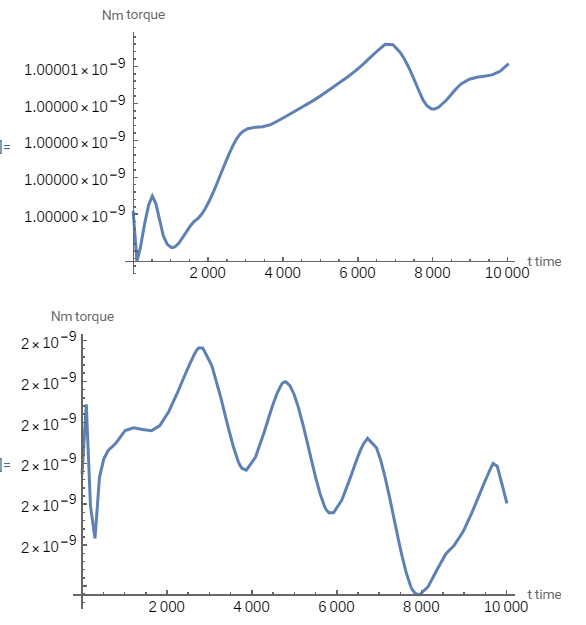
\includegraphics[width=0.8\textwidth]{3_g_t}}[h!]
	We can see that plots are nothing alike so negative Lyapunov exponent can also be coincidence.
\end{document}